\chapter{Cloud-SAP}

\chapterintro{ This chapter introduces the reference architecture known as Cloud-SAP, highlights its core concepts and indicates possible implementation ideas.
}

\section{Motivation}
As one can see, latest advances in providing platform-as-a-service still do not yield a comprehensive solution that embraces a range of fine-grained actions relevant to a given situation in an environment, as it was summarised in previous chapter. All of the presented solutions solely engage horizontal scaling, while other IT processes and corresponding actions such as vertical scaling, cloud bursting or application platform restart remains neglected. What is more, none of the investigated systems is a self-managing one, taking passive approach in enforcing given QoS. To make matter worse, some platforms such as Carina or OneFlow are provider-specific, hence, requiring vast knowledge and time of entities responsible for its supervision.

What system has all of the above-mentioned features is an autonomic one \cite{IBM06}, characterised by a self-management ability and driven by four crucial attributes:
\begin{itemize}
 \item \emph{self-configuration} - dynamic adaptation to changing environment such as provisioning new application instances, application tuning, traffic delegation to an external provider
  \item \emph{self-healing} - discovering, diagnosing and reacting to environment disruption such as container outage
  \item \emph{self-optimising} - monitoring and tuning resources: migrating containers, offloading traffic, for example
  \item \emph{self-protecting} - detecting and protecting against threats such as Deny-of-Service by provisioning extra resources
\end{itemize}

Beside this, key customer values such as IT process execution cost or time needed to complete it are enhanced through rapid process initiation and reduced time and skill requirements \cite{IBM06}. As specified in blueprint, applying autonomic system to manage application environment is possible because following conditions are met:

These four system capabilities combined together yield a promising architecture from QoS ensuring perspective. Beside this, key customer values such as IT process execution cost or time needed to complete it are enhanced through rapid process initiation and reduced time and skill requirements \cite{IBM06}. As specified in blueprint, applying autonomic system to manage application environment is possible because following conditions are met:
\begin{itemize}
  \item tasks involved in associated IT process needs to be automated
  \item it is possible to initiate processes based on observable and detectable situations
  \item autonomic manager posses sufficient knowledge
\end{itemize}

Cloud Self Adaptive Platform (Cloud-SAP) is a reference architecture aspiring to supply application providers with an autonomic computing environment. Figure \ref{img:csap-usage-context} shows Cloud-SAP place in an exemplary application provisioning request. 
\begin{figure}[!ht]
  \begin{center}
    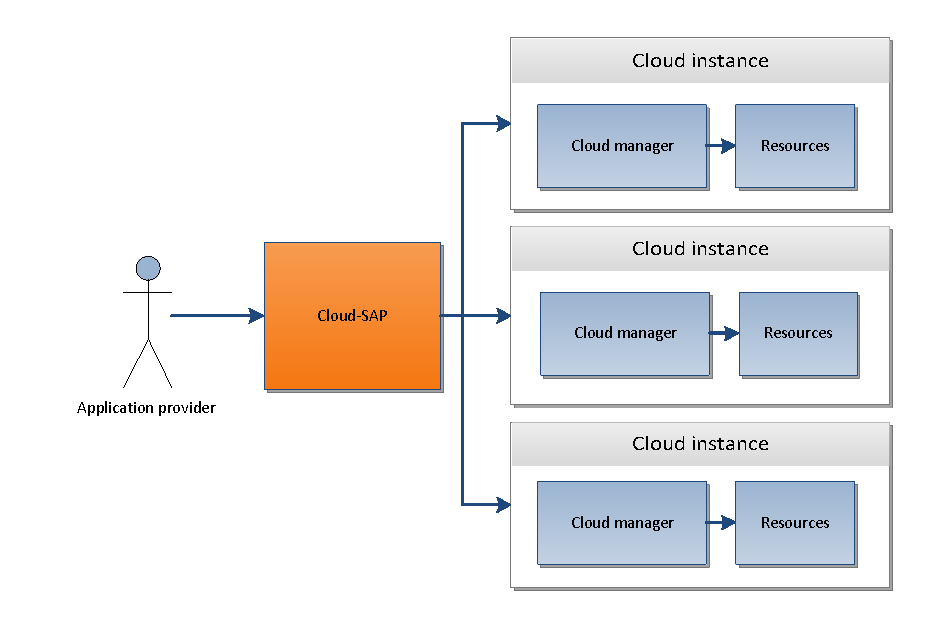
\includegraphics[width=0.9\textwidth]{chapter-design/csap-usage-context}
  \end{center}
  \caption{Cloud-SAP place in an exemplary application provisioning request}
  \label{img:csap-usage-context}
\end{figure}

Application providers can be both end-users or other system interfaces, Cloud-SAP is suitable for both cases. Cloud-SAP is entirely cloud providers and resources agnostic as long as they externalise management interfaces.

Successive sections define core layers of a Cloud-SAP and give insight into possible implementation decisions, while the next chapter presents a proof-of-concept implementation.

\section{Overview}
The previous section dealt with all premises that led to a conclusion that the proposed architecture can rely heavily on the concept of an autonomic system. In this section the further elaboration on the solution is presented.
Figure \ref{img:csap-usage-context} showed the context which the architecture applies to. As one can see, Cloud-SAP can be seen as a proxy between the user and cloud instances and as a coordinator of the latter. Although cloud instance itself consists of a cloud manager and additional resources, in general, it is perfectly legitimate to consider it a resource as well. 

Before the more detailed diagram of the solution is presented, it is essential to introduce another indispensable function that lies in the heart of any autonomic entity -- its ability to detect an undesirable state and take appropriate actions. This is achieved by the presence of a \emph{control loop} which collects data about the environment, analyzes it and takes all needed steps to recover the system. Not only can the attributes introduced in the previous section be bound to an autonomic system, but they can also be thought of main and broad categories of a control loop \cite{IBM06}.

Having said so, we are ready to give a layered overview of a proposed solution, which is shown in figure \ref{img:csap-layered-structure}.
\begin{figure}[!ht]
  \begin{center}
    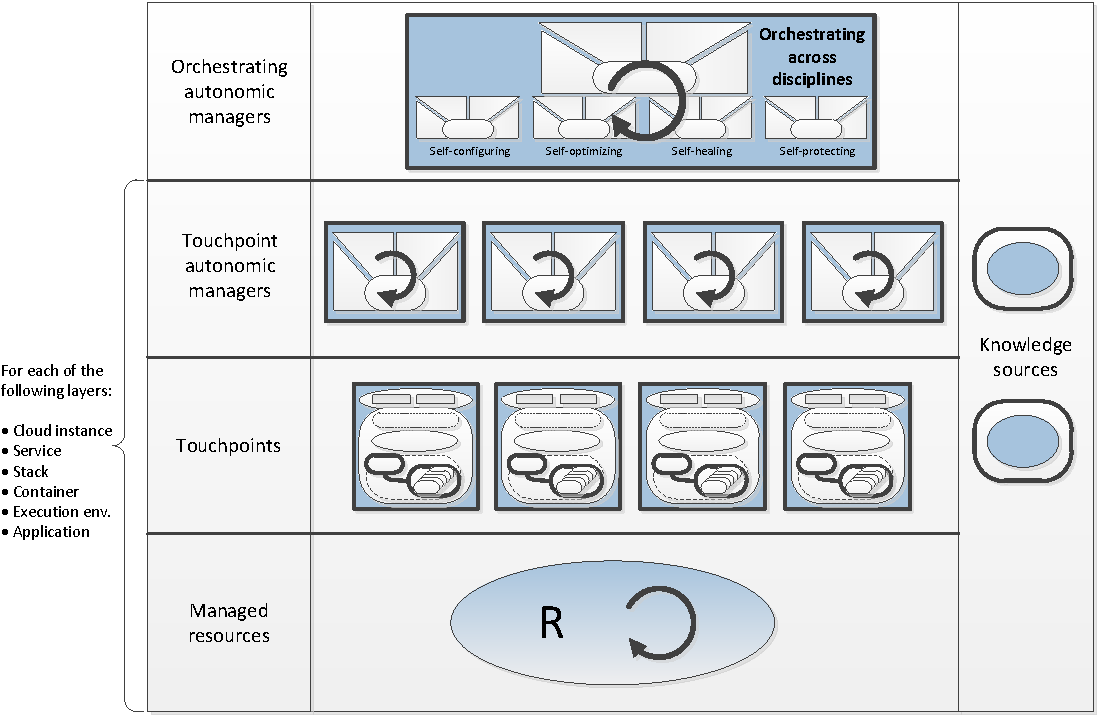
\includegraphics[width=\textwidth]{chapter-design/csap-layers}
  \end{center}
  \caption{Cloud-SAP components seen as IBM autonomic system \cite{IBM06}}
  \label{img:csap-layered-structure}
\end{figure}

The building blocks of the architecture are:
\begin{itemize}
  \item Managed resources
  \item Touchpoints
  \item Touchpoint autonomic managers
  \item Orchestrating autonomic managers
  \item Knowledge source
\end{itemize}
As resources were identified on various levels of abstraction, starting from the application that is to be deployed and ending on a cloud instance that aggregates different applications and services, we can think of the last three layers (managed resources, touchpoints and touchpoint autonomic managers) as a one logical component which can aggregate and manage other components. This recursive definition applies to identified managed resources described in the next section, apart from application as we consider it the most fundamental and indivisible resource.

\subsection{Managed resources}
\emph{Managed resources} form the lowest layer of a stack. When it comes to application provisioning in a cloud environment we can think of the following resources:
\begin{itemize}
  \item \emph{Application} - application itself can be considered resources which can be managed by an external entity, e.g. by restarting/killing it. Interestingly, an application itself can be an autonomic component with an embedded control loop. However, such setting is completely transparent to Cloud-SAP and therefore cannot be managed by it.
  \item \emph{Execution environment of an application} forms an inherent part of an application lifecycle and its proper tuning can greatly influence its performance,
  \item \emph{Container} -- an isolated and controlled environment in which applications are deployed,
  \item \emph{Stack} -- every application has a technology stack associated with it; what is more, if we confine ourselves to map one instance of a container with only one application, we can think of stack as a composition of application (and its execution environment) and a container,
  \item \emph{Service} -- more complex solutions/applications require interactions with various components that are not necessarily implemented using the same technology stack; service denotes a logical entity that consists of a list of stacks that should form one, indivisible component,
  \item \emph{Cloud instance} -- an entity able to deploy \emph{services}
\end{itemize}
What is more, the listed resources are nested within one another and one's ability to work/run smoothly highly depends on the condition and state of the resource it forms part of. This is shown in figure \ref{img:managed-resources-aggregation}.
\begin{figure}[!ht]
  \begin{center}
    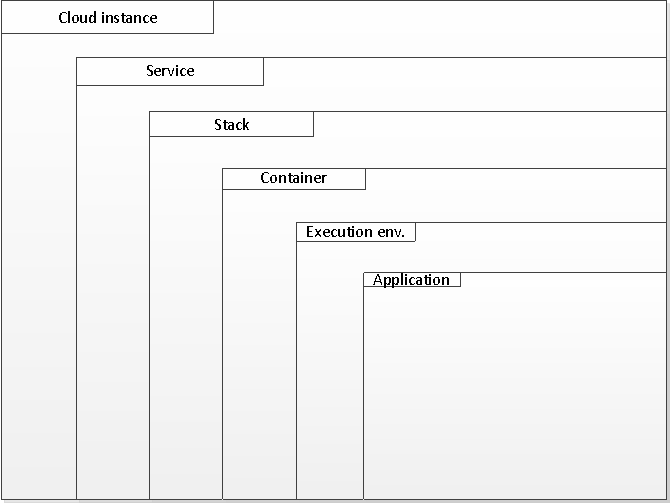
\includegraphics[width=\textwidth]{chapter-design/csap-resources-aggregation}
  \end{center}
  \caption{\emph{Managed resources} identified by Cloud-SAP and their aggregation}
  \label{img:managed-resources-aggregation}
\end{figure}

As it is shown in figure \ref{img:csap-layered-structure}, each \emph{managed resource} can have embedded self-management control loop. The control loop may or may not be externally visible by the manageability interface. For example, an application can have \emph{self-configuring} control loop which performs appropriate runtime tuning of its configuration files, while not being visible (by not providing any API) and manageable by any entity.

\subsection{Touchpoints}
\emph{Touchpoint} forms the layer above managed resources. It has two main functions \cite{IBM06}:
\begin{inparaenum}[1)]
\item provides manageability interface and
\item implements \emph{sensor} and \emph{effector} behaviour.
\end{inparaenum}

By means of manageability interface, external entities can control managed resources. It can be done by, e.g. leveraging API, configuration files or logs. Additionally, it is possible to obtain information via touchpoint about the state of the resource. \emph{Sensor} and \emph{effector} behaviours refers to mechanisms that allows collecting data and change the behaviour of the resource, respectively. Structure of touchpoint is shown in figure \ref{img:csap-touchpoint}.

\begin{figure}[!ht]
  \begin{center}
    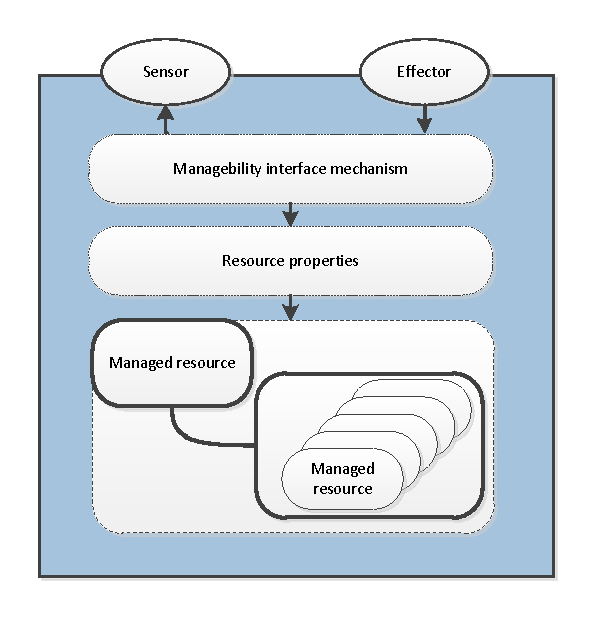
\includegraphics[width=0.7\textwidth]{chapter-design/csap-touchpoint}
  \end{center}
  \caption{Touch point component}
  \label{img:csap-touchpoint}
\end{figure}

\subsection{Touchpoint Autonomic Manager}
\emph{Touchpoint Autonomic Manager} is a component that implements the control loop behaviour and, in effect, manages the managed resources through exposed touchpoints. As it was stated in the previous sections, only four types of control loops are of an interest in the proposed architecture, i.e. \emph{self-configuring}, \emph{self-healing}, \emph{self-optimising} and \emph{self-protecting}.

The actions executed by each control loop on the assigned managed resource are defined in a \emph{policy} that is associated with the given autonomic manager. Thus, there is a one-to-one mapping between managed resource and touchpoint, and touchpoint and autonomic manager.

Each autonomic manager implements the control loop which can be split into four consecutive blocks, which share knowledge among one another. The output from one block forms an input to another. However, it is perfectly possible for a block to perform an action for its side effects, e.g. an action can result in producing relevant information contained in log files, which, in turn, comprises a piece of shared knowledge. Each block implements different behaviour based on the abstraction level and resource they operate on (see figure \ref{img:csap-layered-structure}). Nevertheless it is possible to define their generic behaviour, which embraces the four phases: monitoring, analysis, planning, execution.

\subsubsection{Monitoring}
This function of autonomic manager is responsible for collecting and aggregating data about the resource it manages.  While Cloud-SAP does not have any specific requirements regarding underlying monitoring mechanism, there are a few aspects that should be taken into consideration:
\begin{asparaenum}
  \item[\textbf{Metrics}] Whilst there is a variety of metrics describing resource state, there is no point in monitoring data that client is not interested in. For example, in case when client-defined policies rely entirely on CPU measurements, memory or bandwidth is irrelevant.

  \item[\textbf{Data filters}] Provided that data is gathered from a resource, not all of it should be analysed as some portion of it may be distorted. More specifically, there may be some random spikes in measurements, caused by a temporary process such as garbage collecting. Therefore, Cloud-SAP recommends to transform data using aggregation functions like average, median or filter it by apply low or high-pass filters.

  \item[\textbf{Persistence}] Should collected data be used as a reference point during future control loop iterations, it is persisted, especially along with measures applied by an executor. As a consequence, successive assessments can be more effective by taking into account past symptoms and configuration adjustments. Decision whether to store data in databases, files, external location is entirely left to an implementation.

  \item[\textbf{Standard compatibility}] Whilst there is no single, industry accepted standard of monitoring above-mentioned resources ranging from a single application to whole cloud instance, there were initiatives such as OCCI \cite{OCCI} that aims to close that gap and provide unified view of common appliances. Having scaling across multiple cloud instances in mind, it is vital to provide compatibility at a monitoring level. However, in some cases, standard-defined API may no be sufficient for a specific needs. 
\end{asparaenum}

\subsubsection{Analysis}
This part takes the data from \emph{monitor} phase and performs in-depth analysis of it, which can result in, e.g. prediction plans. It is possible to incorporate more complex mechanisms, such as machine-learning, to fully use the obtained information for better prediction models. For example one or more of the following models can be leveraged \cite{LiWoZh05}:
\begin{asparaenum}
 \item[\textbf{Queue-based performance models}] This models aims to predict QoS measures using resource states and environmental disturbances such as number of service requests. Then a configuration satisfying given QoS is found by a search technique using queues and layered queues. 
 \item[\textbf{Dynamic models}] Aims to represent QoS as a cost function of the difference between the measured value from sensors and set by effectors. Model aspires to minimize that function. Linearized dynamic control is an example of a dynamic model. 
 \item[\textbf{Monotonic static models}] Sought resource state is calculated by discretising a performance model or performing heuristic principles in performance engineering. 
 \item[\textbf{Error correction}] Analysis precision can be improved by applying paddings based on historical data:
    \begin{itemize}
      \item \textit{Burst based padding} - employs a signal processing technique based on fast Fourier transform, burst pattern is extracted and used to calculate a padding value. Coefficients that represents the amplitude of each frequency component are used to calculate burst density. Depending of that value (i.e. is higher than 50\%) appropriate percentile of the burst values are used \cite{ShSuGuWi11}  
      \item \textit{Remedial padding} - padding errors are being recorded and used in successive padding evaluations. In other words, let $e_1, e_2, ... e_k$ denote the recent prediction errors, next the weighted moving average is calculated. Actual applied padding is either padding itself or weighted average, depending which one is greater \cite{ShSuGuWi11}    
    \end{itemize}
 \item[\textbf{Policy based models}] Policy is expressed as a set of constraints that characterise needed resource state. Policies can be categories into two types:
    \begin{itemize}
     \item \emph{Threshold control} - it was already discussed and illustrated in figure \ref{fig:threshold-model}. For example, CPU load can be monitored and when it exceeds a given value, CPU share is increased.
     \item \emph{Policy function control} - a mutli-dimensional extension of a threshold model. It uses multiple variables and control levels \cite{abdeen2002seeking}. It can be further optimised by using Markovian model for a system behaviour \cite{ye2000markov}.     
    \end{itemize}
\end{asparaenum}
Self-learning manager should also use a predictive approach \cite{JiPeLiCh11} and track changes made in a container \cite{ZhYaWo05}. Cloud-SAP requires to at least threshold-model \cite{tong1978threshold} to be supported to enable simple auto-scaling scenario.

\subsubsection{Planning}
During planning phase, procedure to enact desired state of a resource is created. Depending on problem, it may involve only one step such as adjusting one parameter or a more complex like migrating a resource. Before implementing planning module, following issues should be taken into consideration:
\begin{asparaenum}
 \item[\textbf{Priorities}] Multi-tenancy is indispensably correlated with cloud services. As a consequence, resource contends again each other to access to lower-level resources. This can be mitigated by one of the following: \begin{inparaenum}[1)]
    \item avoiding over-provisioning, each tenant has guaranteed resource pool
    \item prioritise tenants, each tenant has assigned priority that indicates its business value; that priority is used to favour one tenant at the expense of the others.
 \end{inparaenum}
 
 \item[\textbf{Reservations}] As previous point indicates, different resources may have different priorities. Therefore, it is suggested to guarantee that most valuable have their QoS requirements satisfied by resource reservation. Inspired by a computer networks, there are at least to ways to retain a certain resource level: 
\begin{inparaenum}[1)]
    \item use parameters such as priority to favour given resource when it is not possible to content every single tenant \cite{nichols1998definition}
    \item secure in advance to retain resource throughout container lifecycle, possibly by using common history patterns \cite{braden1997resource}
 \end{inparaenum}
\end{asparaenum}

\subsubsection{Execution}
The goal of this function of autonomic manager is to execute the planned action

  
What is more, an autonomic manager exposes \emph{sensor} and \emph{effector} manageability interfaces which enables other entities (including other autonomic managers) to manage it in a similar manner as the component itself manages a resource. The image of an autonomic manager with its control loop and provided interface is shown in figure \ref{img:csap-manager}.

\begin{figure}[!ht]
  \begin{center}
    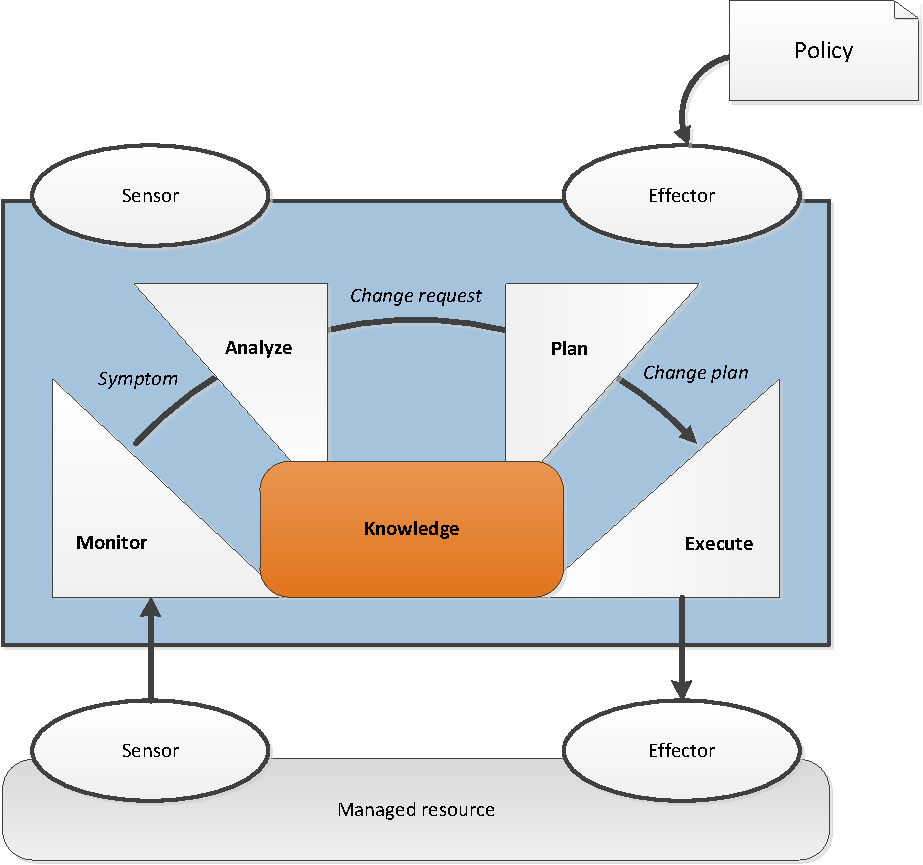
\includegraphics[width=0.7\textwidth]{chapter-design/csap-manager}
  \end{center}
  \caption{Autonomic manager}
  \label{img:csap-manager}
\end{figure}

\subsection{Orchestrating autonomic manager}
While an autonomic manager which manages a single resource may be satisfactory enough in many business cases, there are situations when additional coordination among managers is essential to attain the certain goal. This can result in incorporating autonomic behaviour within an entity in a system-wide scope.

Such a coordination can be achieved by introducing another autonomic manager whose sole purpose is to harmonize the work of dependent ones by extensive use of their \emph{sensor} and \emph{effector} interfaces. These managers are called \emph{orchestrating managers}.

When it comes to the complex task of ensuring the Quality of Service requirements for a client of a cloud computing environment, it is vital to ensure proper mechanisms that would allow seamless cooperation among different cloud providers. Such cooperation could result in a migration of an application between different clouds, market-driven choice of the cloud providers and so on.

As the exemplary actions can be regarded complex ones, they cannot be associated with actions taken by autonomic managers of only one type. Thus, an orchestrating autonomic manager should coordinate other managers of any type -- an arbitrary mixture of self-healing, self-configuring, self-optimizing and self-protecting managers. Employment of these concepts in Cloud-SAP will be discussed later in detail.

\subsection{Knowledge source}
\emph{Knowledge source} provides access to knowledge stored, for example, in a registry, dictionary or database. It is recommended that knowledge source share knowledge among multiple managers, consequently extending their capabilities by performing additional tasks covering recognising particular symptoms or applying specified policies, for instance.


Whilst knowledge can be expressed as symptoms, policies, change requests or history logs, Cloud-SAP differentiates its two main types:
\begin{itemize}
 \item \emph{policy} - set of constraints that, when evaluated, influence system behaviour and possibly trigger further actions. Cloud-SAP does not specify policy format, however, it is vital to employ only one format in whole system so it can be freely exchanged
 \item \emph{problem determination knowledge} - correlation of data, symptoms and decision trees determining actions that can be taken to eliminate symptoms
\end{itemize}

An autonomic manager can obtain knowledge in one of three ways:
\begin{itemize}
 \item \emph{receive it dynamically} - a common way for passing a policy to a manager. 
 \item \emph{retrieve it from external knowledge source} - an approach for obtaining symptom definitions or historical knowledge. For example, detailed history of a resource, its problems and actions taken can be retrieved from a log file.
 \item \emph{create it dynamically} - monitoring and execution phase are strictly correlated and consequently data received from sensors, actions taken by effectors and their result can be stored as a knowledge and provide valuable information during future problem investigations
\end{itemize}


\section{Autonomic execution environment manager}
Autonomic execution environment manager supervises lifecycle of a deployed application's environment by tuning it appropriately to a given usage. More specifically it :
\begin{inparaenum}[1)]
 \item monitors application execution environment i.e. application server
 \item optimises resources used by an application such as thread pool, cache size, databases connections number
 \item restarts application when necessary
\end{inparaenum}

\subsection{Managed resource}
Application execution environment is a set of tools, APIs and frameworks that provides a generalized approach to creating and running an application. It is strictly application specific. In case of java, for example, it can be represented by an application server such as Oracle Weblogic or IBM WebSphere. 

\subsubsection{Touchpoint}
Due to the fact that execution environment is so closely related to a given application type, it is not possible to enlist properties that may be exposed by a touchpoint becouse they vary from application to application. In case of Java EE application touchpoint would externalise management of thread pools, cache and JVM settings such as heap size.

\subsection{Autonomic controller}
Although autonomic controller manages a single resource - an execution environment - it in fact conducts a variety of homogeneous resources - each application type has different properties and consequently vary in actions that can be taken to optimise them. Nevertheless, following subsections presents some common issues and concerns.

\subsubsection{Monitoring}
During monitoring phase, controller collects data from execution environment's touchpoint. Depending on application type it can involve different protocols and APIs. Should one monitor application execution environment, issues and concerns specified in overview are taken into consideration.

\subsubsection{Analysis}
Applying mathematical models to optimise application environment is an exceptionally difficult challenge due to non-linearity of a function denoting dependencies between various parameters. To make matter worse, space of possible solution is unknown and optimal solution heavily depends on a workflow that is tested against. With all that said, models and theories enumerated in an overview can be employed during analysis process. Below is presented a group of such attempts:
\begin{asparaenum}
  \item[\textbf{Smart hill-climbing}] As proposed in \cite{xi2004smart}, application server tuning can be seen as a black-box optimisation problem that can be solved using smart-hill climbing algorithm based on ideas of importance sampling and gradient-based optimisation.

  \item[\textbf{Active Harmony}] This research project uses a simplex method to find the optimal application server parameter settings. Algorithm was validated against a TPC-W benchmark and was proven to optimise application response time by 16\% \cite{chung2004automated}.
\end{asparaenum}


\subsubsection{Planning}
Planning module creates a workflow enacting application environment. It should take into account that different environment requires different procedures and some actions may involve additional tasks such as server restart to be introduced. Besides, some actions interfere with each other and their execution should be planned cautiously. For example changing cache size and cache invalidation interfere with each other and consequently applying this change at same time may not be a good idea.

\subsubsection{Execution}
Finally, controller applies a change plan that tunes the execution environment involving operations such as:
\begin{itemize}
 \item adjusting thread pool
 \item adjusting buffer size
 \item adjusting cache size and its parameters
 \item specifying maximal simultaneous connections
 \item restarting application server
\end{itemize}

% darek
\section{Autonomic container manager}
It is expected that autonomic container manager:
\begin{inparaenum}[1)]
 \item supervises lifecycle of a container: provisions, monitors, migrates and destroys a container
 \item modifies container its properties (i.e. increasing CPU, memory) accordingly to a given condition to ensure that service request are served with a sufficient Quality-of-Service
\end{inparaenum}

\subsection{Managed resource}
To recap, \emph{container} is an entity that provides an execution environment for an application platform. There is a variety of technologies that intend to provide an isolated, secure execution environment. Table \ref{tab:containeristation-technologies} groups them into three main categories: full virtualization, os-level virtualization, operating system process.

\begin{table}[!htbp]
  \centering
  \begin{tabularx}{\textwidth}[]{ X X X X }
    \specialrule{.1em}{.05em}{.05em} 
    & \textbf{Full virtualization} & \textbf{OS-level virtualization} & \textbf{OS process} \\
    \specialrule{.1em}{.05em}{.05em} 
    \textbf{Features} & 
-- complete simulation of machine's hardware

-- full isolation

-- host system is not shared among guests

    &
-- isolation is based on user-spaces

-- shared kernel

-- lesser overhead than full virutalization

-- effective i/o operations
    & 
-- custom solution that uses processes, cgroups, SELinux, for example

-- lesser overhead possible
    
\\ \hline
\textbf{Examples} &
-- KVM

-- Xen

-- VMware &

-- LXC

-- OpenVZ
&
-- OpenShift containers
\\ \hline
  \end{tabularx}
  \caption{Containerisation technologies}
  \label{tab:containeristation-technologies}
\end{table}

While choosing containerisation technique is entirely left to an implementation, Cloud-SAP recommends using os-level virtualization or operating system processes as they involve lesser resources and are more flexible, especially in terms of dynamic adjustment. Moreover, lightweight containers have been proved more effective than full virtualization in some scenarios \cite{RaHiSj13}.

Not only can container be a managed resource but also it can have embedded control loop, depending on chosen mechanism. For example, Xen uses mechanism called 'memory ballooning' to intelligently distribute memory resources among guest systems what is in fact an example of self-optimising control loop. Though, embedded container loops are interesting they does not lie in Cloud-SAP area of interests and as a consequence are not further discussed.

Container uses variety of underlying resources such as storage or network connection. However, for simplicity, Cloud-SAP does not take them into consideration and therefore they are represented merely as a container properties not first-class resources.

\subsubsection{Touchpoint}
Container's touchpoint externalises hypervisor and operating system APIs. Similarly to all touchpoints, sensors for gathering data and effectors for influencing it can be distinguished. It is highly recommended for them to be linked, forming together manageability capabilities. In other words, property (i.e. CPU) can be read only when it is possible to set it as well. For instance, free / used CPU, free / used memory, network bandwidth, disk usage can be measured. Cloud-SAP requires free CPU to be at least supported.

\subsection{Autonomic controller}
\emph{Autonomic container controller} aims to automate container's management function and externalise its configuration through its interfaces. In order to do achieve that, it implements a control loop that fully covers container life cycle. It is suggested for a controller to fully support self-management by implementing \emph{self-configuring, self-healing, self-optimising, self-healing} control loops, however, \emph{self-configuring} is the only one required. Modular structure of a controller is designated by its main four functions: data monitoring, data analysis, action planning and execution along with a knowledge necessary to perform these operations as shown in figure \ref{img:autonomic-component}. 

\subsubsection{Monitoring}
During monitoring phase, controller collects data from container's touchpoint. Issues such as data filtering, aggregation should be taken into consideration as it was stated in overview. 

\subsubsection{Analysis}
Analysis should incorporate prediction techniques and mathematical models specified in overview, producing change requests optimising container behaviour.

\subsubsection{Planning}
This part schedules change requests submitted by an analysis model producing change procedures. Depending on implementation, it may use reservation and priorities mechanisms to enforce given Quality-of-Service level. It vital for a planning phase to be well suited for an underlying hypervisor since not all its types supports dynamic vertical scaling some requires container to be restarted. In that case, container should be cloned and then resized, restarted and finally substitute old, non-scaled instance.

\subsubsection{Execution}
Execution module role is simple yet it plays a role that cannot be underestimated: carrying procedure scheduled beforehand during planning. To do so, it leverages effectors and API exposed by a container. Collectively, these actions scales container vertically, for example:
\begin{itemize}
 \item increase / decrease CPU
 \item increase / decrease memory
 \item increase / decrease disk space
 \item increase / decrease network bandwidth
\end{itemize}
Not every hypervisor supports dynamic vertical scaling, some requires a container to be restared. Noticeably, lightweight containers are flexible in th

In case of a self-learning system, change plan and its effects should be recorded to serve as a reference point in future.

% darek
\section{Autonomic stack manager}
Autonomic stack manager is responsible for a management of a homogeneous resource - containers that together form a stack. More specifically, stack is subjected to:
\begin{inparaenum}[a)]
 \item monitoring its containers
 \item horizontal scaling
 \item changing applied load-balancing algorithms
 \item component replication
\end{inparaenum}

\subsection{Managed resource}
As it was stated in an overview, a stack is a group of containers configured to serve a common purpose (i.e. as a server cluster). In practise, this group consists of a master node and slaves: loadbalancer and java application workers or a master and slave databases, for example. Each stack type may leverage different mechanisms to enable that master-slave relation. Although specific decisions are left to an implementation, chapter X summarises common load-balancing mechanisms.

\subsubsection{Touchpoint}
Stack's touchpoint aims to provide information about the state and condition of a whole group of nodes: master as well as its slaves. As a consequence, from a structural perspective, it is decentralise and consists of a multiple agents. Key properties that should be manageable by a touch point include:
\begin{itemize}
 \item number of service requests passed to a master node
 \item cluster's response time
 \item average cpu / memory usage in cluster
 \item packet loss from all nodes
\end{itemize}

\subsection{Autonomic controller}

\subsubsection{Monitor}
During monitoring phase, controller gathers data from a multiple agents located in stacks' nodes: master and slaves. It is important to ensure that received data is synchronised in time, consequently it can be analysed collectively to find a symptoms covering all of the nodes.

\subsubsection{Analysis}
Analysis phase can be based on one of the models mentioned in an overview. Beside this, following stack and loadbalancing specific models can be taken into consideration:
\begin{asparaenum}
 \item[\textbf{Discrete event simulation model}] It evaluates different balancing algorithms (e.g. round robin, least connection, etc ) to predict which produces least Load-Balancing-Metric (LBM) and packet loss \cite{idziorek2010discrete}.
 \item[\textbf{Optimal static load balancing}] It aims to minimize mean response time of load distributed among servers \cite{tantawi1985optimal}. This model takes into account node's processing time as well as network delays - mean delay time is expressed as weighted sum of them.
 \item[\textbf{Power usage minimisation}] This model is focused on saving computing power by removing computing node when its resource are not necessary. Key assumption is that there is a very little difference in cost of keeping node alive and keeping it 100\% busy. As a consequence nodes should be shut down whenever it is possible \cite{pinheiro2001load}.
\end{asparaenum}


\subsubsection{Planning}
Plan module creates a sequence of changes enacting required QoS. Importantly, produced workflow should minimize or eliminate time during which stack becomes an unavailable due to incorporating additonal slaves or changing load-balancing mechanism, for instance. This can be done using redundant stack or its components to serve requests for a given period of time.

\subsubsection{Execution}
Stack autonomic controller executes actions such as:
\begin{itemize}
 \item horizontal scaling: adding slave nodes
 \item changing load-balancing algorithm
 \item changing network-topology to optimize time needed to reach a stack
 \item replicating master node and hence eliminating SPOF
\end{itemize}



% radek
\section{Autonomic cloud instance manager}
The main responsibility of this manager is the management of a life cycle of resources of a given cloud provider. It could be thought of an autonomic entity which automates the process of managing resources of data centers that forms the services of a cloud instance. The cloud instance manager governs \emph{stacks} of the user-deployed services and its functions include
\begin{inparaenum}[a)]
\item monitoring the state of cloud provider's infrastructure,
\item providing prediction models in terms of resource utilization levels and possible violations of Service Level Agreements,
\item determining the best place (e.g. a physical host) the stack is to be deployed to,
\item ordering a deployment of a stack and
\item migration or eviction of the stacks that do not conform to Quality-of-Service policies provided by the user.
\end{inparaenum}
Additionally, it exposes the manageability interface for taking request from the orchestrating manager.

\subsection{Managed resource}
The resources of a cloud provider can be associated with a data center comprising physical nodes, i.e. clusters, hosts, etc.

\subsubsection*{Touchpoint}
At this level of abstraction, operating system mechanisms and utilities are used to gather information about the state of a given host, e.g. its memory consumption, network throughput and usage statistics, forming the \emph{sensor} behaviour.  Additionally, they are means of performing any changes in the resource what makes them an \emph{effector}.  We want to stress that these features are entirely os-specific and are out of scope of this thesis. For example, there are completely different ways to measure memory usage in Unix/Linux and Windows\texttrademark  environments.

\subsubsection{Monitor}
This function collects information about the data center of a cloud provider. The requirements for this component fall into two categories: resource discovery and information collection.

\begin{asparaenum}
\item[\textbf{Resource discovery}] When a new node is attached to the environment, the function should be able to quickly recognize it and takes it into account in the whole topology of resources comprising the data center.
\item[\textbf{Information collection}] This function gathers and collects nodes' parameters, such as:
  \begin{itemize}
    \item memory (RAM) consumption rate and its attributes (e.g. frequency),
    \item available disk space and other storage parameters (e.g. SSD/HDD),
    \item network type, usage statistics and its attributes such as throughput,
    \item CPU(s) attributes (the number of cores, etc.)
  \end{itemize}
  These parameters are passed to the next function for further analysis.
\end{asparaenum}

\subsubsection{Analyse}
Predictions mechanisms depicted in the \emph{analyse} function of autonomic cloud federation manager applies here as well, so for the clarity of presentation we do not describe it again.

\subsubsection{Plan}
This function aims to solve the problem of an efficient mapping services to available resources so it can be thought of a scheduler of virtual machines within a data center. As in case of other elements of the proposed architecture we do not impose an implementation of a particular solution on an implementer, but we provide a quick overview of available mechanisms and let the final decision be driven by current needs.

One of the approach to this problem is by implementing a Decentralized Online Clustering algorithm \cite{quiroz2009towards}. This solution is an aggregation of virtual machines' provisioning with a workload modeling technique called Quadrature Response Surface Model. It is based on an observation that requests made by a client can be inaccurate and may lead to over-provisioning. The model takes into account also application-specific QoS and SLA requirements.

Constraint Programming can be another method that can be implemented \cite{nguyen2009autonomic} to tackle this problem. This is done by trying to optimize the global utility function of resource provisioning costs and application-specific requirements and constraints. In effect, the management of infrastructure is done in an automated fashion with the effort to reach the maximum performance of hosted applications, keeping the provider's cost at the minimum level at the same time.

\subsubsection{Execute}
The function takes as an input the deployment scheme which has mapped every stack of a service with the given host, irrespective of the use case that triggered the action, i.e. scaling or deployment. The request is delegated to the appropriate stack managers which are responsible for its further processing.

% radek
\section{Autonomic cloud federation manager}
\emph{Autonomic cloud federation manager} is a building block of the proposed architecture that forms the highest layer of its model (see figure \ref{img:csap-layered-structure}). Additionally, it is an element which directly cooperates with a client by capturing and handling their requests.

This manager has two main responsibilities, which include
\begin{inparaenum}[1)]
\item handling deployment of a service requests from the clients and subsequent requests directly applied to that service (e.g. queries about its state), 
\item scaling the previously-deployed service across different cloud vendors.
\end{inparaenum}
The former involves capturing the request from a client, determining the best cloud vendor or vendors for the described service and its deployment. This behaviour is strictly related with \emph{plan} and \emph{execute} functions of an autonomic manager. The latter, on the other hand, involves \emph{monitoring} the dependant autonomic managers that manage in an autonomic fashion cloud instances, \emph{analysing} obtained knowledge and deciding if taking any auto-scaling action is actually necessary to ensure satisfying Quality-of-Service requirements. If such an action is needed, it must be \emph{planned} and \emph{executed}.

The use case of scaling a service withing a federation of cloud vendors can be considered an action which coordinates cloud instance managers. It is perfectly legitimate to view the cloud federation manager as an \emph{orchestrating} one. What is more, such a coordination requires cooperation with not only autonomic managers of a single type, but with the ones that are a mixture of self-healing, self-configuring, self-optimizing and self-protecting. Taking this into account, the orchestration can be classified as an \emph{orchestration across disciplines} \cite{IBM06}.

\subsection{Structure}
It is clear from the description of requirements of this autonomic manager in the previous section that \emph{plan} and \emph{execution} functions are common for both of them. Therefore the \emph{cloud federation manager} is composed of two internal autonomic managers, which perform complete different functions, the first one -- \emph{monitor} and \emph{analyse} and the second -- \emph{plan} and \emph{execute}, yet they cooperate with each other to realize the full control loop.

To be able to handle incoming requests, the manager exposes API a client communicates with. The complete structure of this component is shown in figure \ref{img:orchestrating-autonomic-manager}. In the next sections a detailed description of each internal autonomic manager will be presented.

\begin{figure}[!ht]
  \begin{center}
    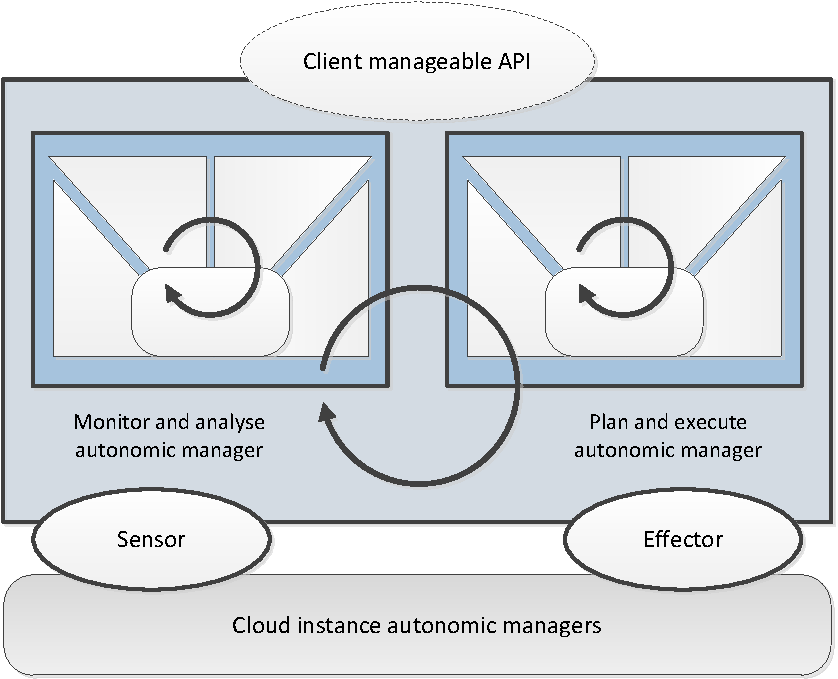
\includegraphics[width=0.7\textwidth]{chapter-design/csap-orchestrating-autonomic-manager}
  \end{center}
  \caption{Design of an orchestrating autonomic manager}
  \label{img:orchestrating-autonomic-manager}
\end{figure}

\subsection{Managed resource}
As it was stated in the previous sections and can be seen in figure \ref{img:orchestrating-autonomic-manager}, \emph{cloud instance autonomic managers} are managed resources of this manager. Each cloud instance is a deployment environment for a service or a stack, i.e. it is possible to span the service across different clouds by deploying stacks which make up the given service to different providers. Of course it is legitimate to deploy the whole service to only one provider.
\subsubsection*{Touchpoints}
As the cloud federation manager has to gain information about the state of a given cloud instance and be able to order the deployment of a stack or a service, the cloud instance exposes its manageability interface and its two types:
\begin{asparaenum}
\item[\textbf{Sensors}] -- set of attributes which forms the state of a given cloud instance. Attributes should include inter alia overall resources usage, pricing, geographical location. The more thorough elaboration will be held in the section devoted to \emph{plan and execution manager}.
\item[\textbf{Effectors}] -- set of stack/service management operations, such as deploy, migrate or delete.
\end{asparaenum}

\subsection{Plan and Execution Autonomic Manager}
The main purpose of this component is to select, based on knowledge provided directly to this manager from \emph{monitor and analyze manager} or a user (i.e. the specification of a service), cloud providers for a given service and carry out the planned action. In the following sections a detailed description of each function is given.

\subsubsection{Plan}
The aim of this function is to give a detailed plan for the action to be performed. In the context of this dissertation the first output produced by this component, regarding the use cases of deploying a service and dynamically scaling it, is a \emph{service deployment plan}, which is a mapping between available resources (cloud instances in this case) and concrete stacks making up the service. The second, definitely less complex, is a queries scheme about the state of the already-deployed services which is based on user's requests. In this case the component only propagates the request to the execute function. As this is only a mediation, there will be no further elaboration on this aspect.

\begin{asparaenum}
  \item[\textbf{Problem description}]
The problem of resource management in cloud computing environments is hard and complex. This is because of several aspects. The first one is the characteristic of resources available in a cloud -- not only are they geographically distributed, but they can be under different administrative domains and can vary in accessibility. This places a heavy burden on cooperation possibilities across cloud providers, both in a technical and non-technical way as providers need to maintain the high level of trust in order to effectively  deliver its products. Additionally, different entities forms the resources -- starting from individual devices, through virtual machines and whole workstations, ending with clusters and data centers. The second one are the increasing Quality-of-Service requirements from the clients. They want resources they use to be reliable, flexible (able to scale according to workload), fault-tolerant, energy-efficient and, of course, cheap. It is clear that clients and cloud vendors have different objectives and supply-and-demand patterns.

There are two main approaches to tackle the problem of effective resource management and scheduling:
  \begin{itemize}
    \item \textbf{conventional style}, in which the mapping decision is determined by some \emph{cost function}. The downside of this method is the fact that in many cases the decision is a function of system-centric parameters \cite{buyya2002economic} and because of it the outcome may lead to better utilization of cloud resources, not necessarily the user's application. What is more, this model treats all resources as if their cost was the same and applications are considered equally important what not always is the case. 

      The positive side of this method is the fact that it involves only one entity that governs the scheduling and allocating the resources. What is more, it is up to the platform how many factors should be incorporated in such a function. Depending on the needs, a more sophisticated or simpler matching algorithm be applied, e.g. an algorithm that takes into account only available budget of a client.
      
      Legion \cite{chapin1999legion} can be an example of a solution which uses this method.
    \item \textbf{economics-paradigm based} \cite{buyya2001case}, in which the decision is not made statically by one entity, but is driven by the users' requirements. The model tries to adopt the real-world economic solution that involves markets and brokers on the computational ground. In this paradigm, clients (representing \emph{demand}) want to solve their problems at the lowest possible price while assuring required Quality-of-Service requirements and constraints, such as time frame. Resource providers (representing \emph{supply}) want to maximise the utilization of their resources while keeping their prices at the level that is attractive for other customers.
      
      Here are the most common economic models which can be applied to resource scheduling and management \cite{buyya2002economic}:
      \begin{itemize}
        \item the commodity market model;
        \item the posted price model;
        \item the bargaining model;
        \item the tendering/contract-net model;
        \item the auction model;
        \item the bid-based proportional resource sharing model;
        \item the community/coalition/bartering model;
        \item the monopoly and oligopoly
      \end{itemize}
  \end{itemize}

\item[\textbf{Function input}] Depending on the actual request, this function can have access to different knowledge that makes its input:

  \begin{asparaenum}
  \item[\textbf{Service deployment}] When the user wants to deploy a service on a cloud infrastructure, they have to prepare its detailed description containing technical (stacks) and Quality-of-Service requirements.
  \item[\textbf{Service scaling}] When an application needs to be scaled, there is available additional knowledge that this component should use of -- detailed information about service's performance up to that point, e.g. service resource utilization level (CPU, I/O), response time, its users profile including their geographical location and so on. This knowledge in a form of a prediction model should be passed to the component by the \emph{analyse} function.
  \end{asparaenum}

\item[\textbf{Function output}] As it was stated in the introductory section, this function produces \emph{service deployment plan}. In the same section we conducted a quick survey of the most common approaches to the resource allocation and mapping problem. The proposed architecture places no restrictions on the chosen approach, as both paradigms can be fitted into it. In the case of \emph{conventional approach}, this component should be equipped with a matching function that takes as an input service description (and the information of its so far execution in the case of an auto-scaling action), offers from cloud providers and make a final decision based on these arguments.
  In the other case, this component can be thought of a cloud exchange \cite{InterCloud10}, that brings together service producers and consumers. Autonomic cloud instance managers could be considered bid-makers and would compete with one another for the client. What is more, if the model is bid-based, the client can have implemented behaviour that would also allow them to participate in auctions. This could be done by introducing another component that would act in user's name.
\end{asparaenum}

\subsubsection{Execute}
This function takes either a query about the state of a service or a deployment plan of the given service and passes execution requests to the proper cloud instance autonomic managers.

\subsection{Monitor and Analyse Autonomic Manager}
\subsubsection*{Introduction}
In many cases designers of applications cannot in advance foresee the detailed requirements of resources of their products, e.g. the number of virtual machines comprising it. This is especially true in case of \emph{start-ups} when it is not known whether the product will catch public attention and who exactly matches the target audience. In such circumstances the cloud provider should be able to quickly adapt to new conditions to prevent the service from being unable to work properly, e.g. take into account the geographical location of the application's users and deploy a service in close proximity to them so as to minimize the latency.

As it was discussed in earlier chapters, the above-mentioned use case refers to \emph{scaling} capabilities of a cloud provider. However, even if a cloud provider has \emph{auto-scaling} mechanisms, there can be unacceptable delays in application response time because of the \emph{reactive} nature of the feature -- the system decides to scale the application based on the \emph{current} resource consumption and utilization rate. Since it involves instantiating and provisioning virtual machines there is always a time overhead associated with it. Hence, there is a need that a system could \emph{predict} demands and behaviours of a hosted service in a \emph{proactive} way. 

The goal of this component is to gather data about current performance of a deployed service and based on it perform an in-depth analysis which results in a resource usage prediction model and auto-scaling schemes. This is the objective of the \emph{monitor} and \emph{analyse} functions, respectively.

\subsubsection*{Prediction models}
One way to divide prediction models into categories is to classify each one as a \emph{reactive} or a \emph{proactive} one. Since in the introductory section there were given reasons why the reactive approach is inefficient, here is a short overview of proactive approaches to the issue.

Using pattern-matching algorithms is one method to tackle the problem and this approach was presented in \cite{caron2010forecasting}. In their work, the algorithm analyses past usage data of an application and tries to identify the most similar patterns to current resource usage characteristics by using a pattern-matching algorithm. Then the obtained patterns are interpolated and the final prediction model is evaluated.

A performance prediction model and only its statistical evaluation is presented in \cite{islam2012empirical}. In that work, the usage of two machine-learning algorithms, \emph{Error Correction Neural Network} and \emph{Linear Regression}, is proposed. Additionally, the authors analyse the problem from an application's provider point of view contrary to most of the work in the field.

An analysis regarding the effectiveness of usage a proactive approach rather than static allocation methods can be found in \cite{kupferman2009scaling}, where a set of scoring metrics is proposed as an efficiency evaluator.

\subsubsection{Monitor}
The main goal of this function is to collect all data regarding usage, performance, resource utilization, capacity and availability of every cloud instance that forms a federation. Further elaboration on the function can be done by aligning use cases of this component:
\begin{asparaenum}
  \item[\textbf{Deployment of a new service}] When a new service is about to be deployed on a cloud federation, the system has to a priori aggregate information about resource capacity, utilization rates, geographical location and so on from cloud providers to be able to perform the best match of a cloud provider with the given service.
  \item[\textbf{Scaling of a deployed service}] When a service which had been hosted on a cloud needs to be scaled, the similar knowledge as in the previous case is required to be passed to \emph{analyse} function to perform the perfect match of a cloud instance.
\end{asparaenum}

The knowledge that the component obtains is about current \emph{topology} (which cloud instances make the cloud federation, what is their geographical location, how are they related, etc.) and \emph{policies} (data required to be compared against policies of deployed serviced). What is more, for the system to be able to perform auto-scaling, the gathered information can be classified as \emph{problem determination knowledge} \cite{IBM06}.

We do not strive to list the data which is required to be collected by this component in a system that tries to conform to the proposed architecture as it completely depends on the system needs. We want to give an overview of possibilities instead and leave the decision to the implementers. The same applies to the components and technology of a persistence layer.

\subsubsection{Analyse}
This function takes knowledge about the cloud federation and a service as an input and outputs a \emph{prediction plan}, which should be helpful in choosing the cloud instance for an application.

In the introductory section a brief overview of some possible techniques and algorithms that can be used in the analyse component was presented. We do not impose a particular method on this component -- it is up to the system complexity and design, which solution would be more suitable to the given needs.

\section{Summary}
Cloud-SAP fills the gap in existing platforms by providing a standardised approach to scaling applications using a fine-grained actions and operating on different platform levels: starting from execution environment and ending on a cloud federation. It is based on a concept of an autonomic system, providing methodical but flexible foundation for its implementation. What is more, Cloud-SAP leverages core benefits of such a system: promise of a self-configuration, self-optimisation, self-health, self-protection. It is driven by a customer-defined policies and consequently ensures that customer is served with demanded Quality-of-Service and with optimised costs.

% TODO Further work?, wady

